\documentclass[letterpaper,11pt,twocolumn]{article}
\usepackage{usenix,graphicx,times,verbatim,enumitem}
\usepackage{graphics, graphicx, fancyhdr, epsfig, amstext}
\usepackage{amsmath, amssymb, xspace, setspace, times, color}
\newtheorem{que}{Question}


\begin{document}

\title{CSCI 339: Distributed Systems --- Project 1 (Web Server)} 
\date{\today}
\author{
  {\rm Daniel Takeshi Seita, Ziang (Lucky) Zhang}\\
       Williams College\\
       \{dts1,zz2\}.@williams.edu
}
\maketitle
\thispagestyle{empty}
%\pagestyle{empty}

\section{Introduction}
A web server listens to connections on a socket to which a client connects. The client can then retrieve files from the server. For instance, a client
can run a web server and use it with Firefox to open up the Williams Computer Science homepage. Alternatively, the client can use \texttt{telnet}
along with  a simple text-based protocol to communicate with the server, which will ideally respond with human-readable messages.

The goal of Project 1 was to build a web server allowing these actions. Our server takes two command line arguments: a document root directory and a
port number. The document root is the directory containing the files that the client can retrieve. Our web server only supports the HTTP GET request,
as that is sufficient to retrieve the contents of a homepage to our server provided that the appropriate files are present in the server's specified
document root directory.

Our server was structured using a \emph{multi-threaded approach} and therefore creates a new thread for each incoming connection.  When a GET request
is sent with the HTTP/1.1 option, after returning results of a request, the server leaves the connection open for some amount of time proportional to
the reciprocal of the number of active threads, so more threads result in a shorter timer.

We also strove to make our server user-friendly. To achieve that, we put some special effort in formatting the server's output. Details and examples
are in in Section~\ref{testing}.

\section{Architectural Overview}

Once our server is running, it continually awaits for connections from clients. When a client connects, the server accepts and spawns a new thread for
dealing with that specific socket while allowing the original thread to listen for additional connections. The server is able to handle over 1000
connections. For a given accepted connection, our server will perform the following steps once the client has sent in a request. Our server detects
this by testing for two carriage returns.

\begin{enumerate}
    \item Our server parses the request to check for correctness. Currently, only GET requests are supported. If the request is incorrectly formatted
according to our rules (explained later), we return a \texttt{400 Bad Request}.
    \item If the client made an appropriately formatted GET request, we extract the requested file name and search for it. If it is not found, or if
the client does not have the correct permissions, we return \texttt{404 Not Found} and \texttt{403 Forbidden}, respectively.
    \item If the file can be found and read, our server sends a response back to the client that includes the contents of the file, as well as HTTP
headers and status codes.
    \item After responding to the client, the server closes the connection if it was using HTTP/1.0, but keeps the connection open for a bit longer if
using HTTP/1.1. 
\end{enumerate}

Each of these steps above is described in more detail in the following subsections.

\subsection{Parsing the Request}

Our server checks the initial request line from the client to see if it starts out with: \texttt{GET [directory] HTTP/\{1.0, 1.1\}}.\footnote{The brackets at
the end mean either 1.0 or 1.1 can be appended.} It does so by extracting the line, splitting it based on whitespace (multiple whitespace are
allowed), and checks the first and third tokens. If any of its checks fail, it sends a \texttt{400 Bad Request}. Otherwise, it extracts the file name
from the second token, which is the \texttt{[directory]}, and calls a procedure to validate the file. Additional text after the three tokens is
allowed because clients could decide to send more information.

\subsection{Checking the File}

With a given file path, the server first checks to make sure no instance of \texttt{../} is found in the path, since this would mean the client might
be accessing parent (or other) files outside the server's document root. The server outputs a 404 error if this happens; otherwise, it moves on to
checking the file status. We first use the \texttt{stat} function with the file path as input to check for existence, and then used the
\texttt{S\_IROTH} flag to check for file permissions. If either of these checks fail, the server outputs the appropriate error message, which is 404
or 403, respectively. If the file is deemed to exist and is readable, then the server moves on to sending a response.

\subsection{The Server's Response}

The server's response includes the following elements: the HTTP status codes, the date, the content type, the content length, the server name, and
finally, the requested file itself. At this point, the server responds with an \texttt{HTTP/\{1.0,1.1\} 200 OK} message, since it did not output any
earlier status codes that would have indicated failure. (Our server implements the 200, 400, 403, 404, and 500 status codes.) It then prints the
\texttt{Date} header, which displays the current date in the following form: \texttt{[DayOfWeek] [Month] [Day] [Hours:Mins:Secs] [Year] ([UTC Time])}.
The UTC Time is included so that no one has to try and guess the time zone.

Following that, the server prints out the \texttt{Content-Type} header. It detects the type of the file by extracting the file extension from the file
name. Currently supported file types are \texttt{html/txt}, \texttt{jpg}, and \texttt{gif}. The server then prints out \texttt{Content-Length}, which
uses \texttt{fseek} to determine the number of bytes of data in the file, and then \texttt{Server}, which is the highly creative name \texttt{Daniel
and Lucky's Server}.

Finally, the actual file is printed!

\subsection{HTTP/1.0 and HTTP/1.1}

If the client's GET request includes HTTP/1.0, then the server simply closes the connection after sending its response. Things get more interesting if
using HTTP/1.1, because now the server will keep the connection open longer, avoiding the overhead of commencing and closing TCP connection. It keeps
the connection open for a thread until its timer goes to zero. Our timeout heuristic makes the server close faster if it is servicing more requests.
The formula for computing a given timer is to divide a constant variable by the number of active threads, i.e. $constTime /(\#\:threads)$. (In our
experiments, we set the constant to be 300 seconds.) If a given connection has received a request from the client, the server responds and then resets
the timer back to $constTime /(\#\:threads)$, though the number of threads may have changed while this was happening, so the timer is not guaranteed to
be the same as it was before the request. We use a global variable to count the number of active threads and protect it with a lock to prevent race
conditions.

\subsection{Addendum: Using Threads}

We designed our server to create multiple threads for each connection. Of the three major design options available to us (multi-threaded,
multi-processed, and event-driven), we decided that using threads was the simplest and cleanest way to achieve our goals, especially since we were
building and testing the server using basic GET requests from a web browser. We did not see any need to create extra, bulky processors, and vastly
preferred low communication context switching and overhead. The risk is with shared resources, but the only item we needed to protect was the count of
the number of threads active.



\section{Some Problems Encountered}\label{problems}

There were several challenging aspects of this project. One was being able to determine how to even get started. Fortunately, the socket programming
tutorial from the University of Massachusetts that was provided on the CSCI 339 project website got us up and running with a single-socket server that
successfully sent files.

We also did not initially implement re-usability of ports (and sockets). This caused a problem because it created situations when we could successfully
run our server on port, say, 8101, and then after closing the server and immediately re-starting it using the exact same command, it would not start!
Fortunately, Jeannie directed us to the \texttt{setsockopt} function, which allowed us to reuse ports. Her emails also led us to the right direction
in timing out our sockets, which were among the last features we implemented.

\section{Examples and Testing}\label{testing}

In this section, we go over how to use our server and some sample client-server responses. Figure~\ref{start} shows the process of compiling the
server with \texttt{make}, along with a specified document directory. One can immediately see the start of our user-friendly server messages, which
clearly explains to the user that the server is binded and ready to accept connections.

\begin{figure}[t]
  \centering
   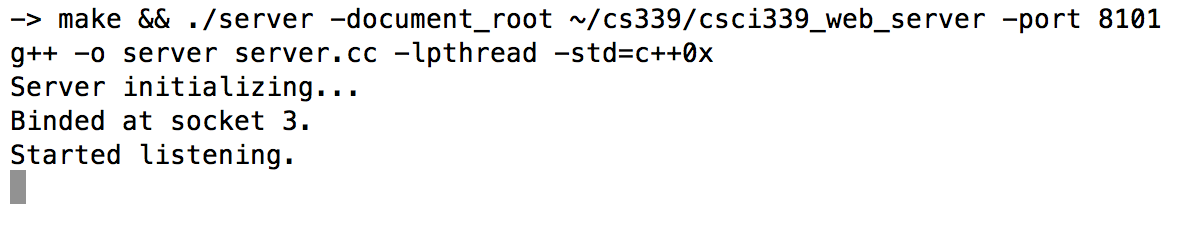
\includegraphics[width=\columnwidth]{example1.png}     
  \caption{Compiling and running a server.\label{start}}
\end{figure} 

Now consider when the user connects to the server via \texttt{telnet} and the appropriate port number. Upon successful connection, the user can type
in a GET request for a file. This process is shown in Figure~\ref{request}, with the requested file as \texttt{index2.html}. This is a simple file
containing just one line: \texttt{THIS IS DANIEL!}. The text of the file is shown in the server's response after the appropriate headers: the HTTP
status code, the date, the content type, the content length, and the server's name. Notice here that the connection closes immediately after the
server's response. Had the request been for HTTP 1.1, the conneciton would remain until the timer ran out.

\begin{figure}[t]
  \centering
   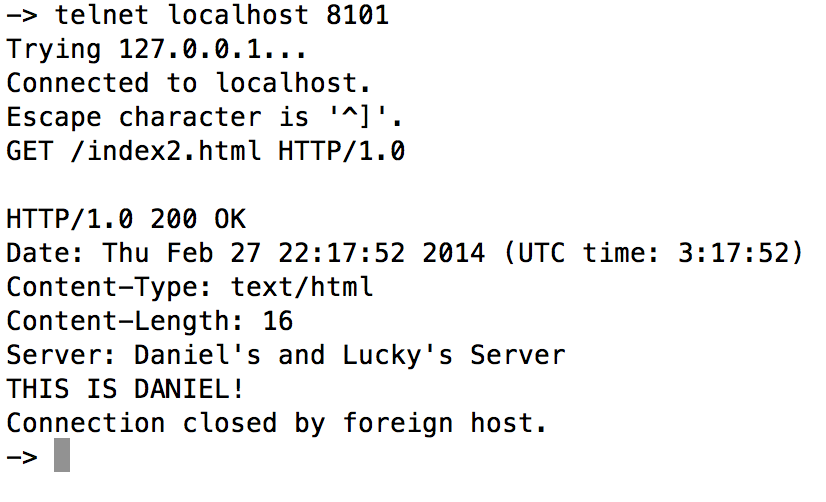
\includegraphics[width=\columnwidth]{example2.png}     
  \caption{What the user sees while connecting to our server.\label{request}}
\end{figure} 

Naturally, if we have bad requests, our server should output error messages. While all this is happening, our server is printing out user-friendly
messages. A partial segment is shown in Figure~\ref{output}

\begin{figure}[t]
  \centering
   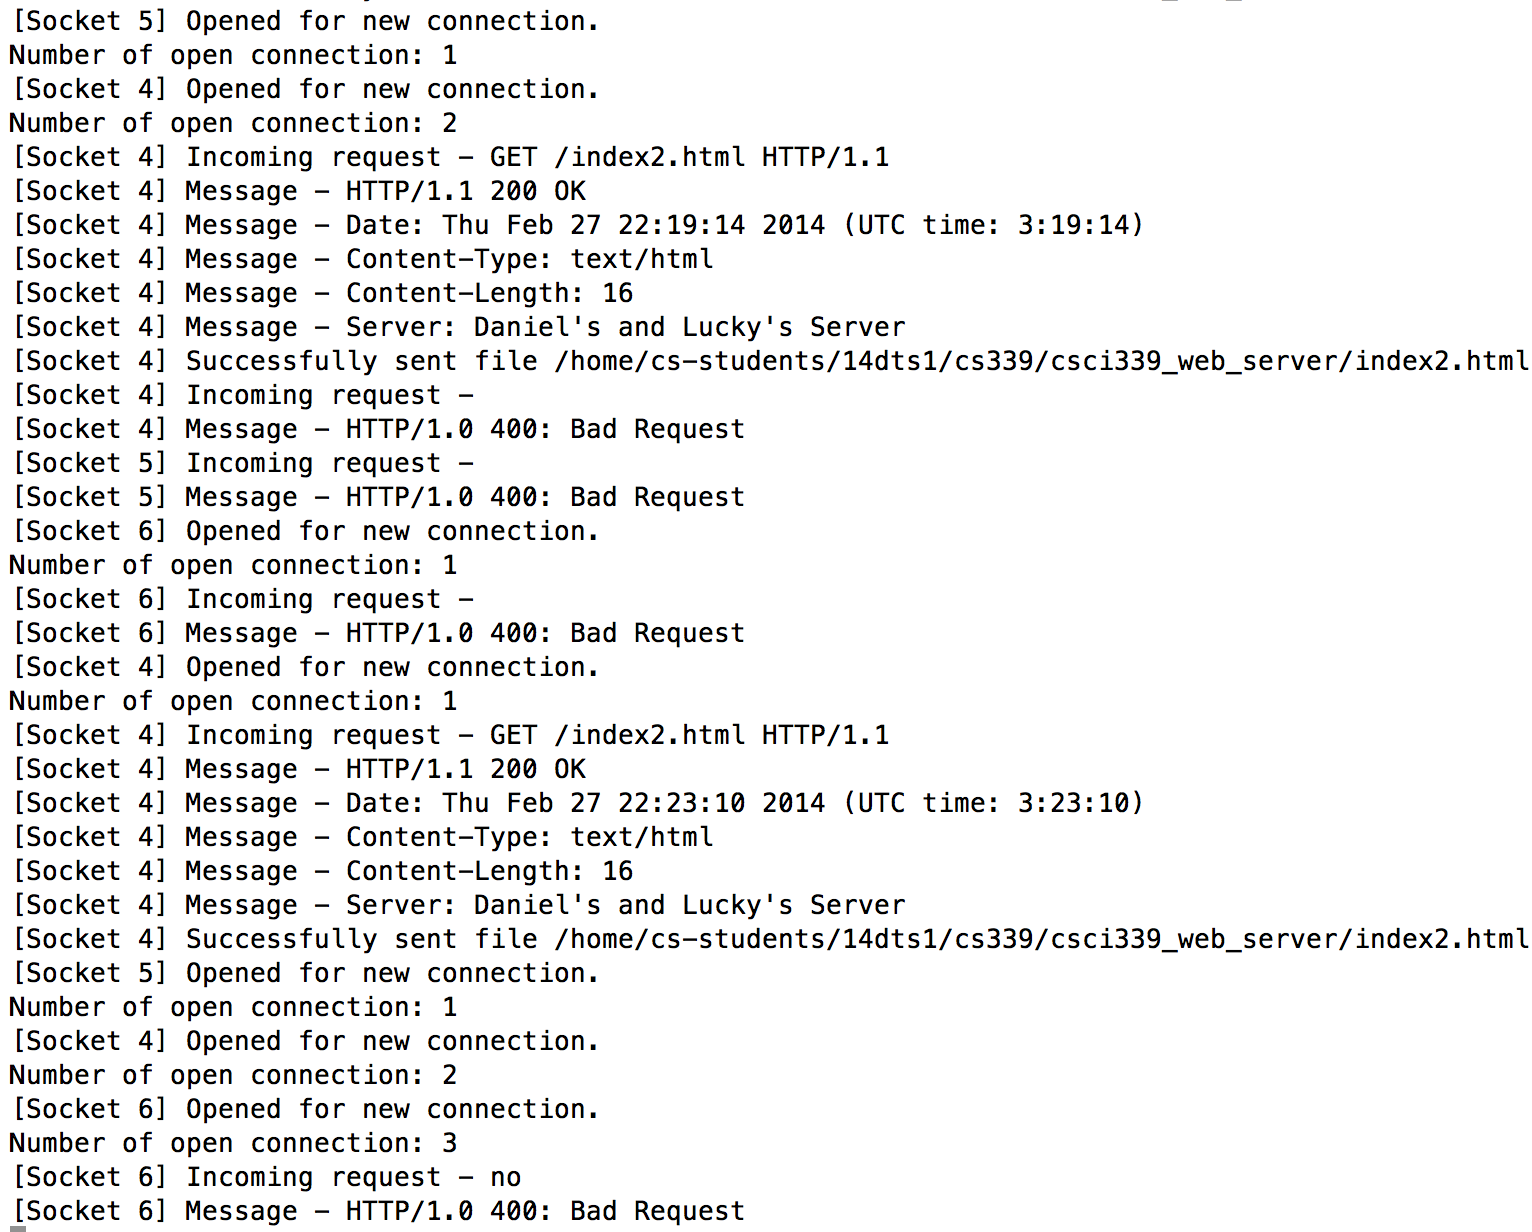
\includegraphics[width=\columnwidth]{example3.png}     
  \caption{Examples of output from our server, including some examples of bad requests.\label{output}}
\end{figure} 


\section{Questions}\label{questions}

\begin{que}
Although it wasn't required, how would you go about supporting .htaccess in your server? 
\end{que}

These \texttt{.htaccess}es are text files used to control how a web server can access files in a directory. If our web server had supported these
files, then for each file request, it would first extract the IP address of the user. Then, it needs to check the paths leading up to the requested
file for \texttt{.htaccess} files to make sure they exist and that they allow clients with that IP address to access it. To change our code, we would
parse the file path name by directory (i.e., by the ``/'' character) and then search sequentially in each directory up to the one containing the
actual file itself. Naturally, we return an error and terminate the connection at any point in this process.

\begin{que}
Can you think of a scenario in which HTTP/1.0 may perform better than HTTP/1.1? Can you think of a scenario when HTTP/1.1 outperforms HTTP/1.0?
\end{que}

HTTP/1.0 generally works well when the benefits of immediate parallelism outperform the cost of the slow start and establishing/destroying the TCP
connection. One scenario when it would work well would be when the server must send some enormous files and is experiencing significant latency and
low bandwidth. In that case, using a single connection per session might not be wise because each one of the gigantic files must be (slowly) processed
in order, and the startup and connection costs are lower compared to the cost of the entire session. Thus, HTTP/1.0 is probably better in this case.

What if the server were instead dealing with a large amount of small files, with high bandwidth and low latency. In this hypothetical case, it might
make more sense to use HTTP/1.1 to avoid the comparatively more expensive startup and TCP connection costs required by a purely multi-threaded
approach that makes a new connection per object. The high bandwidth means each object is processed quickly, which keeps the pipeline moving.

One certainly needs to consider the tradeoffs if the situation is ``in between'' these extreme cases, but the above examples should hopefully capture
some obvious reasons to use HTTP/1.0 or HTTP/1.1.

\section{Conclusion}\label{conclusion}
This was an interesting first project. We started out slow as we spent some time reading over the (very helpful) references given on the assignments
page. As mentioned in Section~\ref{problems}, the tutorial on socket programming got us started. Following that, we implemented some of the more minor
details, such as generating appropriate HTTP responses, before moving on to managing multiple connections/threads and creating a timeout for the
HTTP/1.1 option. The end result is a server that we hope is completely functional, allows multiple clients to connect, correctly implements a timeout
to reflect HTTP/1.0 and HTTP/1.1 differences, is user-friendly, can work on multiple browsers (we tested on Firefox and Google Chrome) and is free of
unknown bugs.

% No bibliography for this document.
%\bibliographystyle{plain}
%\bibliography{bibfile}


\begin{comment}
Here we describe the design of our system. Figures are sometimes helpful.  
We can discuss the key design choices we made, and provide support and
justification for why we made these choices.

The following text demonstrates how to include an eps figure in your
document.  It also shows the usefulness of ``verbatim'' text in LaTeX:

\begin{verbatim}
\begin{figure}[t]
  \centering
   \includegraphics[width=\columnwidth]{sword-arch.pdf}     
  \caption{This is how we insert 
           an eps figure.
           \label{sword-arch}}
\end{figure} 
\end{verbatim}
\end{comment}

\end{document}
